% Compile with pdflatex to preview every figure of the paper (TikZ/pgfplots sources in figures/).
\documentclass[a4paper]{article}
\usepackage[margin=1.8cm]{geometry}
\usepackage{amsmath,amssymb}
\usepackage{tikz}
\usetikzlibrary{positioning,arrows.meta,fit,backgrounds,calc}
\usepackage{pgfplots}
\usepgfplotslibrary{groupplots,fillbetween}
\pgfplotsset{compat=1.18}
\definecolor{cAllon}{HTML}{8A8984}
\definecolor{cET}{HTML}{EB6834}
\definecolor{cETH}{HTML}{7A3FC2}
\definecolor{cSFCT}{HTML}{D6559A}
\definecolor{cWang}{HTML}{B38600}
\definecolor{cOurs}{HTML}{2A78D6}
\definecolor{cOracle}{HTML}{0B0B0B}
\definecolor{cViol}{HTML}{E34948}
\definecolor{cCode}{HTML}{1BAF7A}
\definecolor{cLoad}{HTML}{6250D6}
\definecolor{cBg}{HTML}{EB6834}
\definecolor{cLeaf}{HTML}{C9C8C2}

\begin{document}
\section*{fig\_trace}
% generated by gen_figures.py -- do not edit by hand
\pgfplotsset{conap/.style={
  width=\linewidth, scale only axis=false, tick label style={font=\scriptsize}, label style={font=\scriptsize},
  title style={font=\scriptsize\bfseries, at={(0,1)}, anchor=south west, inner sep=1pt},
  legend style={font=\scriptsize, draw=none, fill=none}, grid=major, grid style={gray!20},
  axis line style={gray!70}, tick style={gray!70}, every axis plot/.append style={line join=round}}}
\begin{tikzpicture}
\begin{axis}[conap, width=0.80\linewidth, height=4.0cm, xmin=0, xmax=9, ymin=0, ymax=950,
  ylabel={KV transfer demand (Gbps)}, xtick={0,2,4,6,8}, xticklabels={May 10,May 12,May 14,May 16,May 18},
  axis y line*=left, legend columns=3, legend style={at={(0.5,1.02)}, anchor=south, /tikz/every even column/.append style={column sep=4pt}}]
\addlegendimage{cViol, line width=1.6pt}\addlegendentry{Network power}
\addplot[cOurs, line width=0.6pt] coordinates {(2,105.1) (2.02083,111.9) (2.04167,111.7) (2.0625,121.3) (2.08333,114.9) (2.10417,108.6) (2.125,103.2) (2.14583,97.4) (2.16667,96.9) (2.1875,89.7) (2.20833,101.5) (2.22917,94.9) (2.25,103.2) (2.27083,104.2) (2.29167,116.0) (2.3125,119.2) (2.33333,117.5) (2.35417,116.8) (2.375,109.9) (2.39583,109.1) (2.41667,111.3) (2.4375,114.0) (2.45833,122.1) (2.47917,128.7) (2.5,125.1) (2.52083,135.8) (2.54167,161.8) (2.5625,160.6) (2.58333,148.6) (2.60417,146.5) (2.625,148.3) (2.64583,153.3) (2.66667,146.9) (2.6875,137.3) (2.70833,148.9) (2.72917,139.8) (2.75,146.0) (2.77083,144.0) (2.79167,131.4) (2.8125,136.4) (2.83333,131.1) (2.85417,133.8) (2.875,137.6) (2.89583,120.7) (2.91667,120.5) (2.9375,120.2) (2.95833,134.0) (2.97917,164.0) (3,191.1) (3.02083,207.6) (3.04167,222.8) (3.0625,235.3) (3.08333,234.5) (3.10417,232.8) (3.125,192.0) (3.14583,182.4) (3.16667,186.5) (3.1875,197.7) (3.20833,198.3) (3.22917,222.9) (3.25,233.2) (3.27083,249.3) (3.29167,237.6) (3.3125,254.5) (3.33333,265.1) (3.35417,250.6) (3.375,235.0) (3.39583,220.1) (3.41667,225.9) (3.4375,229.8) (3.45833,238.8) (3.47917,233.7) (3.5,235.1) (3.52083,254.4) (3.54167,268.0) (3.5625,287.0) (3.58333,295.5) (3.60417,308.3) (3.625,287.5) (3.64583,277.9) (3.66667,242.8) (3.6875,245.1) (3.70833,228.6) (3.72917,228.2) (3.75,225.0) (3.77083,223.5) (3.79167,207.5) (3.8125,238.1) (3.83333,228.3) (3.85417,200.1) (3.875,170.7) (3.89583,179.4) (3.91667,173.3) (3.9375,170.5) (3.95833,179.6) (3.97917,194.8) (4,210.0) (4.02083,226.7) (4.04167,219.2) (4.0625,239.0) (4.08333,249.0) (4.10417,238.3) (4.125,198.5) (4.14583,188.7) (4.16667,199.4) (4.1875,197.8) (4.20833,207.9) (4.22917,224.9) (4.25,234.1) (4.27083,260.0) (4.29167,269.5) (4.3125,272.5) (4.33333,274.1) (4.35417,253.0) (4.375,248.5) (4.39583,247.9) (4.41667,222.0) (4.4375,236.0) (4.45833,243.5) (4.47917,257.5) (4.5,273.5) (4.52083,283.4) (4.54167,273.0) (4.5625,302.7) (4.58333,312.9) (4.60417,313.0) (4.625,309.1) (4.64583,276.4) (4.66667,268.4) (4.6875,267.5) (4.70833,249.5) (4.72917,246.9) (4.75,262.8) (4.77083,262.3) (4.79167,248.3) (4.8125,238.4) (4.83333,235.2) (4.85417,210.9) (4.875,187.3) (4.89583,195.7) (4.91667,179.0) (4.9375,153.2) (4.95833,147.2) (4.97917,178.0) (5,190.2) (5.02083,209.1) (5.04167,217.9) (5.0625,218.1) (5.08333,217.1) (5.10417,212.8) (5.125,182.3) (5.14583,175.6) (5.16667,188.2) (5.1875,210.9) (5.20833,202.0) (5.22917,219.9) (5.25,226.7) (5.27083,249.7) (5.29167,252.5) (5.3125,254.5) (5.33333,253.6) (5.35417,241.9) (5.375,236.1) (5.39583,243.3) (5.41667,228.1) (5.4375,211.5) (5.45833,219.8) (5.47917,230.6) (5.5,250.2) (5.52083,254.0) (5.54167,259.5) (5.5625,291.4) (5.58333,289.8) (5.60417,268.7) (5.625,268.9) (5.64583,259.2) (5.66667,240.5) (5.6875,235.4) (5.70833,208.4) (5.72917,230.1) (5.75,234.1) (5.77083,224.8) (5.79167,219.4) (5.8125,214.3) (5.83333,188.8) (5.85417,186.5) (5.875,152.6) (5.89583,136.8) (5.91667,136.0) (5.9375,143.7) (5.95833,150.7) (5.97917,177.7) (6,194.6) (6.02083,211.1) (6.04167,218.9) (6.0625,223.7) (6.08333,232.1) (6.10417,230.0) (6.125,193.6) (6.14583,179.1) (6.16667,191.6) (6.1875,181.2) (6.20833,182.7) (6.22917,221.5) (6.25,239.7) (6.27083,256.6) (6.29167,246.0) (6.3125,273.6) (6.33333,275.2) (6.35417,272.5) (6.375,264.4) (6.39583,245.8) (6.41667,201.0) (6.4375,200.5) (6.45833,202.0) (6.47917,217.3) (6.5,216.0) (6.52083,242.9) (6.54167,269.5) (6.5625,266.5) (6.58333,272.0) (6.60417,279.2) (6.625,239.5) (6.64583,242.3) (6.66667,224.3) (6.6875,214.6) (6.70833,209.3) (6.72917,217.0) (6.75,221.4) (6.77083,207.1) (6.79167,203.0) (6.8125,191.3) (6.83333,178.5) (6.85417,171.4) (6.875,164.9) (6.89583,144.7) (6.91667,141.0) (6.9375,137.8) (6.95833,151.0) (6.97917,169.3) (7,200.9) (7.02083,226.9) (7.04167,226.8) (7.0625,234.6) (7.08333,238.0) (7.10417,214.9) (7.125,189.9) (7.14583,178.1) (7.16667,190.0) (7.1875,195.8) (7.20833,214.1) (7.22917,221.2) (7.25,229.6) (7.27083,250.0) (7.29167,260.3) (7.3125,256.4) (7.33333,247.4) (7.35417,240.7) (7.375,247.0) (7.39583,234.9) (7.41667,221.7) (7.4375,193.6) (7.45833,196.0) (7.47917,197.8) (7.5,211.4) (7.52083,220.8) (7.54167,237.5) (7.5625,233.3) (7.58333,222.0) (7.60417,240.0) (7.625,215.7) (7.64583,222.2) (7.66667,199.7) (7.6875,199.3) (7.70833,198.5) (7.72917,186.0) (7.75,164.8) (7.77083,174.5) (7.79167,153.4) (7.8125,162.5) (7.83333,156.0) (7.85417,150.6) (7.875,131.1) (7.89583,125.3) (7.91667,111.9) (7.9375,112.7) (7.95833,105.0) (7.97917,114.6) (8,106.1) (8.02083,117.0) (8.04167,123.2) (8.0625,114.0) (8.08333,125.4) (8.10417,120.9) (8.125,101.3) (8.14583,106.0) (8.16667,103.2) (8.1875,99.2) (8.20833,110.6) (8.22917,107.7) (8.25,109.9) (8.27083,117.3) (8.29167,121.6) (8.3125,130.4) (8.33333,135.7) (8.35417,128.4) (8.375,122.3) (8.39583,103.8) (8.41667,119.9) (8.4375,124.4) (8.45833,127.8) (8.47917,140.4) (8.5,146.6) (8.52083,146.3) (8.54167,155.7) (8.5625,139.8) (8.58333,153.8) (8.60417,165.1) (8.625,171.3) (8.64583,157.2) (8.66667,157.9) (8.6875,150.1) (8.70833,150.0) (8.72917,137.6) (8.75,121.3) (8.77083,129.9) (8.79167,119.5) (8.8125,119.6) (8.83333,130.5) (8.85417,128.5) (8.875,113.7) (8.89583,126.1) (8.91667,99.9) (8.9375,112.5) (8.95833,106.6) (8.97917,103.7)};
\addlegendentry{Conversation}
\addplot[cCode, line width=0.6pt] coordinates {(0,146.6) (0.0208333,131.6) (0.0416667,125.5) (0.0625,126.1) (0.0833333,124.2) (0.104167,113.1) (0.125,97.7) (0.145833,109.8) (0.166667,97.6) (0.1875,81.8) (0.208333,72.0) (0.229167,66.0) (0.25,58.8) (0.270833,62.7) (0.291667,55.9) (0.3125,56.0) (0.333333,49.5) (0.354167,49.6) (0.375,59.7) (0.395833,54.0) (0.416667,52.9) (0.4375,56.4) (0.458333,66.1) (0.479167,77.7) (0.5,108.1) (0.520833,158.3) (0.541667,194.4) (0.5625,242.5) (0.583333,298.2) (0.604167,362.8) (0.625,374.0) (0.645833,358.7) (0.666667,337.1) (0.6875,345.8) (0.708333,375.4) (0.729167,384.0) (0.75,403.8) (0.770833,402.3) (0.791667,397.1) (0.8125,458.4) (0.833333,426.7) (0.854167,381.9) (0.875,312.6) (0.895833,271.8) (0.916667,222.3) (0.9375,196.0) (0.958333,150.5) (0.979167,121.5) (1,105.1) (1.02083,94.5) (1.04167,91.9) (1.0625,81.8) (1.08333,74.4) (1.10417,77.5) (1.125,82.6) (1.14583,71.8) (1.16667,67.2) (1.1875,64.4) (1.20833,53.5) (1.22917,46.3) (1.25,42.2) (1.27083,44.6) (1.29167,33.4) (1.3125,27.7) (1.33333,25.1) (1.35417,24.2) (1.375,21.2) (1.39583,20.2) (1.41667,17.9) (1.4375,17.0) (1.45833,25.6) (1.47917,28.7) (1.5,36.6) (1.52083,42.8) (1.54167,46.5) (1.5625,64.5) (1.58333,67.3) (1.60417,80.9) (1.625,72.4) (1.64583,81.1) (1.66667,78.9) (1.6875,82.2) (1.70833,91.2) (1.72917,90.4) (1.75,92.4) (1.77083,111.6) (1.79167,110.6) (1.8125,103.1) (1.83333,92.0) (1.85417,96.6) (1.875,88.2) (1.89583,80.9) (1.91667,82.1) (1.9375,89.2) (1.95833,80.2) (1.97917,68.5) (2,71.8) (2.02083,72.3) (2.04167,72.8) (2.0625,87.1) (2.08333,75.4) (2.10417,68.6) (2.125,70.9) (2.14583,71.6) (2.16667,63.8) (2.1875,58.3) (2.20833,53.6) (2.22917,47.5) (2.25,43.2) (2.27083,38.8) (2.29167,29.0) (2.3125,23.9) (2.33333,23.0) (2.35417,24.8) (2.375,23.9) (2.39583,20.7) (2.41667,22.8) (2.4375,22.5) (2.45833,21.4) (2.47917,26.9) (2.5,31.3) (2.52083,45.6) (2.54167,48.7) (2.5625,51.1) (2.58333,54.1) (2.60417,60.3) (2.625,64.3) (2.64583,63.6) (2.66667,67.7) (2.6875,75.9) (2.70833,70.6) (2.72917,75.8) (2.75,83.9) (2.77083,90.6) (2.79167,88.7) (2.8125,85.3) (2.83333,85.4) (2.85417,93.5) (2.875,99.7) (2.89583,104.2) (2.91667,97.6) (2.9375,84.9) (2.95833,95.3) (2.97917,100.4) (3,113.3) (3.02083,103.1) (3.04167,103.3) (3.0625,115.9) (3.08333,122.3) (3.10417,105.4) (3.125,98.0) (3.14583,100.8) (3.16667,88.3) (3.1875,77.7) (3.20833,69.9) (3.22917,75.9) (3.25,67.2) (3.27083,67.2) (3.29167,62.2) (3.3125,66.1) (3.33333,51.8) (3.35417,57.0) (3.375,54.0) (3.39583,57.1) (3.41667,53.9) (3.4375,54.5) (3.45833,67.5) (3.47917,94.1) (3.5,114.7) (3.52083,154.7) (3.54167,213.9) (3.5625,301.3) (3.58333,315.3) (3.60417,425.4) (3.625,413.3) (3.64583,425.9) (3.66667,380.8) (3.6875,410.9) (3.70833,416.5) (3.72917,461.9) (3.75,494.3) (3.77083,517.1) (3.79167,530.2) (3.8125,536.3) (3.83333,525.5) (3.85417,491.5) (3.875,408.9) (3.89583,351.7) (3.91667,300.1) (3.9375,284.0) (3.95833,219.2) (3.97917,175.1) (4,173.5) (4.02083,188.2) (4.04167,168.6) (4.0625,176.3) (4.08333,158.8) (4.10417,154.7) (4.125,118.7) (4.14583,99.1) (4.16667,95.0) (4.1875,87.5) (4.20833,72.9) (4.22917,73.1) (4.25,62.0) (4.27083,69.9) (4.29167,60.9) (4.3125,58.4) (4.33333,57.6) (4.35417,59.1) (4.375,70.0) (4.39583,62.7) (4.41667,68.3) (4.4375,68.5) (4.45833,78.8) (4.47917,100.7) (4.5,146.1) (4.52083,190.1) (4.54167,269.9) (4.5625,344.5) (4.58333,403.9) (4.60417,451.1) (4.625,477.3) (4.64583,455.7) (4.66667,377.6) (4.6875,426.2) (4.70833,437.2) (4.72917,520.0) (4.75,541.4) (4.77083,583.9) (4.79167,577.5) (4.8125,552.9) (4.83333,555.4) (4.85417,507.0) (4.875,374.7) (4.89583,349.5) (4.91667,271.6) (4.9375,253.0) (4.95833,210.8) (4.97917,164.5) (5,179.4) (5.02083,158.0) (5.04167,140.6) (5.0625,150.8) (5.08333,146.9) (5.10417,138.0) (5.125,142.5) (5.14583,121.3) (5.16667,108.4) (5.1875,91.4) (5.20833,81.5) (5.22917,84.7) (5.25,74.0) (5.27083,81.9) (5.29167,67.9) (5.3125,61.2) (5.33333,62.7) (5.35417,59.6) (5.375,55.2) (5.39583,57.3) (5.41667,62.8) (5.4375,71.7) (5.45833,77.1) (5.47917,98.5) (5.5,140.4) (5.52083,198.6) (5.54167,257.2) (5.5625,330.0) (5.58333,366.0) (5.60417,404.2) (5.625,431.2) (5.64583,470.8) (5.66667,438.8) (5.6875,462.5) (5.70833,477.7) (5.72917,531.0) (5.75,535.1) (5.77083,574.6) (5.79167,581.9) (5.8125,581.1) (5.83333,606.4) (5.85417,538.0) (5.875,457.3) (5.89583,351.1) (5.91667,275.7) (5.9375,229.9) (5.95833,197.6) (5.97917,200.5) (6,171.3) (6.02083,156.9) (6.04167,142.7) (6.0625,148.7) (6.08333,141.5) (6.10417,149.4) (6.125,133.2) (6.14583,103.1) (6.16667,94.9) (6.1875,91.3) (6.20833,91.4) (6.22917,72.4) (6.25,79.6) (6.27083,72.5) (6.29167,65.6) (6.3125,63.6) (6.33333,57.8) (6.35417,64.3) (6.375,61.9) (6.39583,65.9) (6.41667,59.6) (6.4375,67.5) (6.45833,85.7) (6.47917,109.5) (6.5,151.4) (6.52083,205.4) (6.54167,243.8) (6.5625,288.5) (6.58333,359.7) (6.60417,432.3) (6.625,421.7) (6.64583,429.2) (6.66667,390.2) (6.6875,463.4) (6.70833,461.1) (6.72917,508.1) (6.75,515.5) (6.77083,555.8) (6.79167,527.0) (6.8125,547.1) (6.83333,521.2) (6.85417,477.5) (6.875,379.6) (6.89583,332.8) (6.91667,270.6) (6.9375,223.1) (6.95833,191.1) (6.97917,181.1)};
\addlegendentry{Coding}
\end{axis}
\begin{axis}[conap, width=0.80\linewidth, height=4.0cm, xmin=0, xmax=9, ymin=0, ymax=125, axis y line*=right, axis x line=none,
  ylabel={Network power (\% of peak)}, ylabel style={cViol}, yticklabel style={cViol}, grid=none]
\addplot[cViol, line width=1.6pt] coordinates {(0,100) (9,100)};
\end{axis}
\end{tikzpicture}

\clearpage
\section*{fig\_topology}
% Detailed data-plane topology: (a) scale-out leaf--spine fabric, (b) inside one server.
% Example symmetric configuration c = (w,u,r,e) = (2,4,400,4).
\resizebox{\textwidth}{!}{%
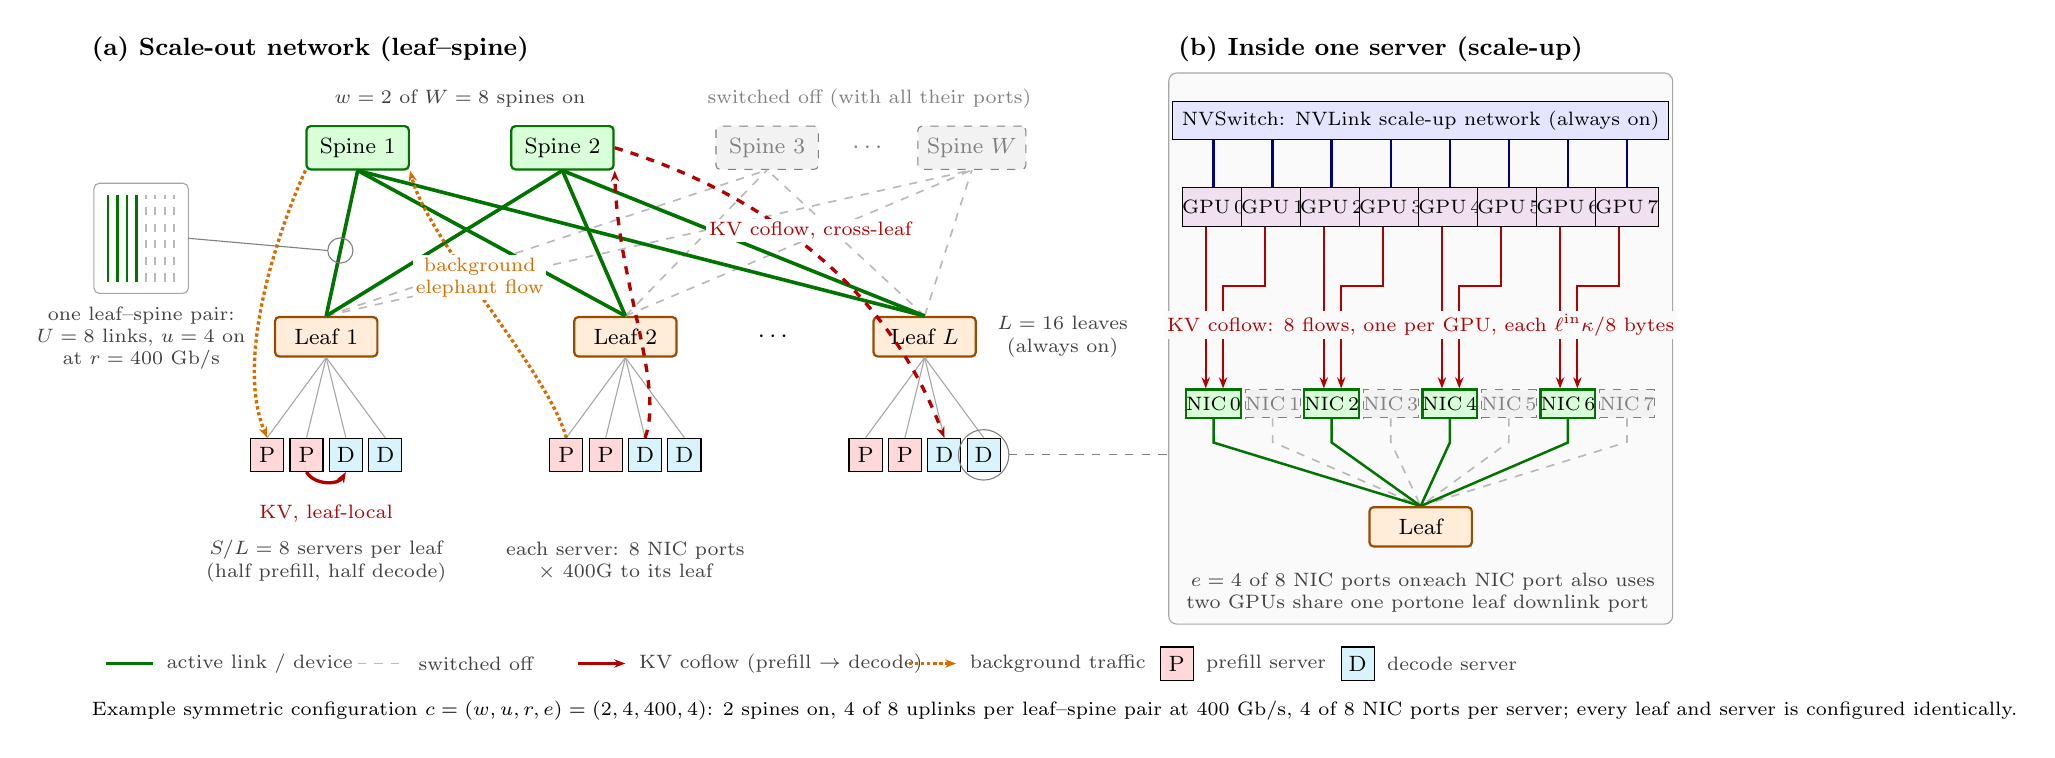
\begin{tikzpicture}[
  font=\footnotesize, >={Stealth[length=4pt]},
  spon/.style={draw=green!45!black, fill=green!15, rounded corners=1.5pt, minimum width=1.3cm, minimum height=0.55cm, thick},
  spoff/.style={draw=gray, fill=gray!10, text=gray, dashed, rounded corners=1.5pt, minimum width=1.3cm, minimum height=0.55cm},
  leaf/.style={draw=orange!60!black, fill=orange!15, rounded corners=1.5pt, minimum width=1.3cm, minimum height=0.5cm, thick},
  srvP/.style={draw, fill=red!15, minimum width=0.42cm, minimum height=0.42cm, inner sep=0pt},
  srvD/.style={draw, fill=cyan!15, minimum width=0.42cm, minimum height=0.42cm, inner sep=0pt},
  upon/.style={green!45!black, line width=1.3pt},
  upoff/.style={gray!55, dashed, line width=0.6pt},
  gpu/.style={draw, fill=violet!12, minimum width=0.66cm, minimum height=0.5cm, inner sep=0pt, font=\scriptsize},
  nicon/.style={draw=green!45!black, fill=green!15, thick, minimum width=0.66cm, minimum height=0.36cm, inner sep=0pt, font=\scriptsize},
  nicoff/.style={draw=gray, fill=gray!10, text=gray, dashed, minimum width=0.66cm, minimum height=0.36cm, inner sep=0pt, font=\scriptsize},
  kv/.style={red!70!black, very thick, ->},
  bg/.style={orange!85!black, very thick, ->, densely dotted},
  note/.style={font=\scriptsize, align=center, text=black!75}]

% =========================== (a) scale-out fabric ===========================
\node[font=\small\bfseries, anchor=west] at (-1.5,7.25) {(a) Scale-out network (leaf--spine)};

\node[spon]  (S1) at (2.0,6.0) {Spine 1};
\node[spon]  (S2) at (4.6,6.0) {Spine 2};
\node[spoff] (S3) at (7.2,6.0) {Spine 3};
\node[font=\small, gray] at (8.5,6.0) {$\cdots$};
\node[spoff] (SW) at (9.8,6.0) {Spine $W$};
\node[note] at (3.3,6.62) {$w=2$ of $W=8$ spines on};
\node[note, text=gray] at (8.5,6.62) {switched off (with all their ports)};

\node[leaf] (L1) at (1.6,3.6) {Leaf 1};
\node[leaf] (L2) at (5.4,3.6) {Leaf 2};
\node[font=\small] at (7.3,3.6) {$\cdots$};
\node[leaf] (LL) at (9.2,3.6) {Leaf $L$};
\node[note, anchor=west] at (10.0,3.6) {$L=16$ leaves\\ (always on)};

\foreach \l in {L1,L2,LL}{
  \foreach \s in {S3,SW}{\draw[upoff] (\l.north) -- (\s.south);}
  \foreach \s in {S1,S2}{\draw[upon] (\l.north) -- (\s.south);}
}

% zoom on one leaf--spine bundle
\coordinate (zc) at ($(L1.north)!0.45!(S1.south)$);
\draw[gray] (zc) circle (0.16);
\begin{scope}[shift={(-0.75,4.85)}]
  \draw[gray!70, rounded corners=2pt, fill=white] (-0.6,-0.7) rectangle (0.6,0.7);
  \foreach \i in {0,...,3}{\draw[upon, line width=0.8pt] (-0.42+0.12*\i,-0.55) -- (-0.42+0.12*\i,0.55);}
  \foreach \i in {4,...,7}{\draw[upoff] (-0.42+0.12*\i,-0.55) -- (-0.42+0.12*\i,0.55);}
  \node[note, anchor=north] at (0,-0.75) {one leaf--spine pair:\\ $U=8$ links, $u=4$ on\\ at $r=400$ Gb/s};
\end{scope}
\draw[gray] (-0.15,4.85) -- ($(zc)+(-0.16,0)$);

% servers
\foreach \l/\x in {L1/1.6, L2/5.4, LL/9.2}{
  \node[srvP] (\l p1) at (\x-0.75,2.1) {P};
  \node[srvP] (\l p2) at (\x-0.25,2.1) {P};
  \node[srvD] (\l d1) at (\x+0.25,2.1) {D};
  \node[srvD] (\l d2) at (\x+0.75,2.1) {D};
  \foreach \s in {p1,p2,d1,d2}{\draw[gray!70] (\l\s.north) -- (\l.south);}
}
\node[note] at (1.6,0.75) {$S/L=8$ servers per leaf\\ (half prefill, half decode)};
\node[note] at (5.4,0.75) {each server: 8 NIC ports\\ $\times$ 400G to its leaf};

% KV coflow inside one leaf
\draw[kv] (L1p2.south) to[bend right=60] (L1d1.south);
\node[note, text=red!70!black] at (1.6,1.35) {KV, leaf-local};
% KV coflow across leaves via spine 2
\draw[kv, dashed] (L2d1.north) .. controls (5.9,3.0) and (5.3,4.3) .. (S2.south east);
\draw[kv, dashed] (S2.east) .. controls (6.6,5.6) and (8.6,4.6) .. (LLd1.north);
\node[note, text=red!70!black, fill=white, inner sep=1pt] at (7.75,4.95) {KV coflow, cross-leaf};
% background elephant flow via spine 1
\draw[bg] (L2p1.north) .. controls (4.4,3.2) and (2.9,4.8) .. (S1.south east);
\draw[bg] (S1.south west) .. controls (1.1,5.2) and (0.4,3.4) .. (L1p1.north);
\node[note, text=orange!85!black, fill=white, inner sep=1pt] at (3.55,4.35) {background\\ elephant flow};

% =========================== (b) inside one server ===========================
\node[font=\small\bfseries, anchor=west] at (12.3,7.25) {(b) Inside one server (scale-up)};
\draw[rounded corners=3pt, fill=gray!4, draw=gray!70] (12.3,-0.05) rectangle (18.7,6.95);
\node[draw, fill=blue!10, minimum width=5.9cm, minimum height=0.45cm, font=\scriptsize] (NVS) at (15.5,6.35) {NVSwitch: NVLink scale-up network (always on)};
\foreach \i in {0,...,7}{
  \node[gpu] (G\i) at (12.87+0.75*\i,5.25) {GPU\,\i};
  \draw[blue!50!black, line width=0.9pt] (G\i.north) -- (G\i.north |- NVS.south);
}
\foreach \i in {0,2,4,6}{\node[nicon]  (N\i) at (12.87+0.75*\i,2.75) {NIC\,\i};}
\foreach \i in {1,3,5,7}{\node[nicoff] (N\i) at (12.87+0.75*\i,2.75) {NIC\,\i};}
% PCIe paths: with e = 4, GPUs 2k and 2k+1 share NIC 2k
\foreach \k in {0,2,4,6}{
  \pgfmathtruncatemacro{\j}{\k+1}
  \draw[kv, line width=0.8pt] ($(G\k.south)+(-0.1,0)$) -- ($(N\k.north)+(-0.1,0)$);
  \draw[kv, line width=0.8pt] ($(G\j.south)+(-0.1,0)$) -- ++(0,-0.75) -| ($(N\k.north)+(0.12,0)$);
}
\node[note, text=red!70!black, fill=gray!4, inner sep=1pt] at (15.5,3.75) {KV coflow: 8 flows, one per GPU, each $\ell^{\rm in}\kappa/8$ bytes};
% links to the leaf
\coordinate (leafin) at (15.5,1.45);
\foreach \i in {1,3,5,7}{\draw[upoff] (N\i.south) -- ++(0,-0.3) -- (leafin);}
\foreach \i in {0,2,4,6}{\draw[upon, line width=0.9pt] (N\i.south) -- ++(0,-0.3) -- (leafin);}
\node[leaf, anchor=north] (Lz) at (leafin) {Leaf};
\node[note, anchor=west] at (12.4,0.35) {$e=4$ of 8 NIC ports on:\\ two GPUs share one port};
\node[note, anchor=east] at (18.6,0.35) {each NIC port also uses\\ one leaf downlink port};

% zoom link from (a) to (b)
\draw[gray] (LLd2) circle (0.32);
\draw[gray, dashed] ($(LLd2)+(0.32,0)$) -- (12.3,2.1);

% =========================== legend ===========================
\begin{scope}[shift={(-1.2,-0.55)}]
  \draw[upon] (0,0) -- (0.6,0); \node[note, anchor=west] at (0.65,0) {active link / device};
  \draw[upoff] (3.2,0) -- (3.8,0); \node[note, anchor=west] at (3.85,0) {switched off};
  \draw[kv] (6.0,0) -- (6.6,0); \node[note, anchor=west] at (6.65,0) {KV coflow (prefill $\to$ decode)};
  \draw[bg] (10.2,0) -- (10.8,0); \node[note, anchor=west] at (10.85,0) {background traffic};
  \node[srvP] at (13.6,0) {P}; \node[note, anchor=west] at (13.85,0) {prefill server};
  \node[srvD] at (15.9,0) {D}; \node[note, anchor=west] at (16.15,0) {decode server};
\end{scope}
\node[anchor=west, font=\scriptsize] at (-1.5,-1.15) {Example symmetric configuration $c=(w,u,r,e)=(2,4,400,4)$: 2 spines on, 4 of 8 uplinks per leaf--spine pair at 400 Gb/s, 4 of 8 NIC ports per server; every leaf and server is configured identically.};
\end{tikzpicture}%
}

\clearpage
\section*{fig\_saving}
% generated by gen_figures.py -- do not edit by hand
\pgfplotsset{conap/.style={
  width=\linewidth, scale only axis=false, tick label style={font=\scriptsize}, label style={font=\scriptsize},
  title style={font=\scriptsize\bfseries, at={(0,1)}, anchor=south west, inner sep=1pt},
  legend style={font=\scriptsize, draw=none, fill=none}, grid=major, grid style={gray!20},
  axis line style={gray!70}, tick style={gray!70}, every axis plot/.append style={line join=round}}}
\begin{tikzpicture}
\begin{groupplot}[conap, group style={group size=2 by 1, horizontal sep=0.9cm}, width=0.47\textwidth, height=4.2cm,
  ymin=0, ymax=82, xmin=-0.6, xmax=5.6, xtick={0,...,5}, ymajorgrids, xmajorgrids=false,
  xticklabels={ElasticTree,ET+Hedera,SmartFCT-like,Wang22-like,CoNap (ours),Oracle}, xticklabel style={rotate=40, anchor=north east, font=\scriptsize}]
\nextgroupplot[title={(a) base}, ylabel={Saving vs.\ All-on (\%)}]
\addplot[ybar, bar width=9pt, fill=cET, draw=white] coordinates {(0,34.9)};
\node[font=\scriptsize\bfseries, text=cViol, anchor=south] at (axis cs:0,34.9) {24};
\addplot[ybar, bar width=9pt, fill=cETH, draw=white] coordinates {(1,34.9)};
\node[font=\scriptsize, text=black, anchor=south] at (axis cs:1,34.9) {1};
\addplot[ybar, bar width=9pt, fill=cSFCT, draw=white] coordinates {(2,35.6)};
\node[font=\scriptsize\bfseries, text=cViol, anchor=south] at (axis cs:2,35.6) {5};
\addplot[ybar, bar width=9pt, fill=cWang, draw=white] coordinates {(3,36.8)};
\node[font=\scriptsize\bfseries, text=cViol, anchor=south] at (axis cs:3,36.8) {12};
\addplot[ybar, bar width=9pt, fill=cOurs, draw=white] coordinates {(4,68.3)};
\node[font=\scriptsize, text=black, anchor=south] at (axis cs:4,68.3) {0};
\addplot[ybar, bar width=9pt, fill=cOracle, draw=white] coordinates {(5,69.9)};
\node[font=\scriptsize, text=black, anchor=south] at (axis cs:5,69.9) {0};
\nextgroupplot[title={(b) kvheavy}]
\addplot[ybar, bar width=9pt, fill=cET, draw=white] coordinates {(0,39.1)};
\node[font=\scriptsize\bfseries, text=cViol, anchor=south] at (axis cs:0,39.1) {24};
\addplot[ybar, bar width=9pt, fill=cETH, draw=white] coordinates {(1,39.1)};
\node[font=\scriptsize\bfseries, text=cViol, anchor=south] at (axis cs:1,39.1) {24};
\addplot[ybar, bar width=9pt, fill=cSFCT, draw=white] coordinates {(2,3.0)};
\node[font=\scriptsize\bfseries, text=cViol, anchor=south] at (axis cs:2,3.0) {2};
\addplot[ybar, bar width=9pt, fill=cWang, draw=white] coordinates {(3,39.1)};
\node[font=\scriptsize\bfseries, text=cViol, anchor=south] at (axis cs:3,39.1) {24};
\addplot[ybar, bar width=9pt, fill=cOurs, draw=white] coordinates {(4,60.9)};
\node[font=\scriptsize, text=black, anchor=south] at (axis cs:4,60.9) {0};
\addplot[ybar, bar width=9pt, fill=cOracle, draw=white] coordinates {(5,61.1)};
\node[font=\scriptsize, text=black, anchor=south] at (axis cs:5,61.1) {0};
\end{groupplot}
\end{tikzpicture}

\clearpage
\section*{fig\_tail}
% generated by gen_figures.py -- do not edit by hand
\pgfplotsset{conap/.style={
  width=\linewidth, scale only axis=false, tick label style={font=\scriptsize}, label style={font=\scriptsize},
  title style={font=\scriptsize\bfseries, at={(0,1)}, anchor=south west, inner sep=1pt},
  legend style={font=\scriptsize, draw=none, fill=none}, grid=major, grid style={gray!20},
  axis line style={gray!70}, tick style={gray!70}, every axis plot/.append style={line join=round}}}
\begin{tikzpicture}
\begin{groupplot}[conap, group style={group size=2 by 2, horizontal sep=0.9cm, vertical sep=0.35cm, x descriptions at=edge bottom},
  width=0.47\textwidth, height=3.4cm, xmin=0, xmax=24, xtick={0,4,...,24},
  legend columns=6, legend style={/tikz/every even column/.append style={column sep=5pt}}]
\nextgroupplot[ymin=0, ymax=15, title={(a) base}, ylabel={P99 slowdown}, legend to name=legtail]
\addplot[draw=none, fill=cViol, fill opacity=0.10, forget plot] coordinates {(0,8.792) (24,8.792) (24,15) (0,15)} -- cycle;
\addplot[cViol, line width=0.6pt, forget plot] coordinates {(0,8.792) (24,8.792)};
\node[font=\tiny, text=cViol, anchor=north east] at (axis cs:23.8,15) {SLO violated};
\addplot[cAllon, solid, line width=0.6pt] coordinates {(0.5,5.8614) (1.5,5.2007) (2.5,5.0000) (3.5,5.2841) (4.5,5.0000) (5.5,5.0000) (6.5,4.1990) (7.5,4.8652) (8.5,4.0000) (9.5,4.3437) (10.5,4.1129) (11.5,4.7337) (12.5,4.0000) (13.5,3.9985) (14.5,4.0000) (15.5,4.0376) (16.5,4.0000) (17.5,4.2695) (18.5,4.0000) (19.5,4.5540) (20.5,4.0000) (21.5,4.5419) (22.5,4.2143) (23.5,4.0061)};
\addlegendentry{All-on}
\addplot[cET, dashed, line width=0.7pt] coordinates {(0.5,12.6418) (1.5,11.3962) (2.5,11.5318) (3.5,9.7908) (4.5,9.5086) (5.5,10.0197) (6.5,10.0739) (7.5,10.0000) (8.5,11.7742) (9.5,12.0539) (10.5,13.0000) (11.5,11.8333) (12.5,9.9975) (13.5,9.4459) (14.5,11.0632) (15.5,9.1905) (16.5,10.7861) (17.5,11.4895) (18.5,10.6081) (19.5,11.4032) (20.5,11.0000) (21.5,10.2318) (22.5,11.5505) (23.5,12.0000)};
\addlegendentry{ElasticTree}
\addplot[cETH, dashed, line width=0.7pt] coordinates {(0.5,4.2656) (1.5,4.0000) (2.5,4.0000) (3.5,3.0000) (4.5,3.0000) (5.5,3.9234) (6.5,4.0772) (7.5,4.0000) (8.5,6.4619) (9.5,5.5078) (10.5,5.4148) (11.5,5.8147) (12.5,5.1349) (13.5,4.8707) (14.5,5.2326) (15.5,4.5267) (16.5,5.0000) (17.5,5.4282) (18.5,5.0000) (19.5,5.0854) (20.5,5.1618) (21.5,4.8306) (22.5,4.9883) (23.5,5.2982)};
\addlegendentry{ET+Hedera}
\addplot[cSFCT, dash dot, line width=0.7pt] coordinates {(0.5,14.0000) (1.5,6.6431) (2.5,7.8489) (3.5,6.6688) (4.5,6.5400) (5.5,6.9552) (6.5,7.3047) (7.5,8.8523) (8.5,8.1275) (9.5,8.1713) (10.5,6.5845) (11.5,8.2178) (12.5,7.6767) (13.5,7.0152) (14.5,7.7728) (15.5,8.2367) (16.5,7.4146) (17.5,7.8056) (18.5,9.6644) (19.5,7.9862) (20.5,7.8328) (21.5,6.0655) (22.5,7.9237) (23.5,9.0000)};
\addlegendentry{SmartFCT-like}
\addplot[cWang, densely dotted, line width=0.9pt] coordinates {(0.5,4.2656) (1.5,4.0000) (2.5,4.0000) (3.5,4.0000) (4.5,4.2012) (5.5,3.9234) (6.5,4.0772) (7.5,5.8687) (8.5,6.4619) (9.5,5.5078) (10.5,8.9148) (11.5,9.0074) (12.5,8.2467) (13.5,7.7110) (14.5,8.8342) (15.5,7.3862) (16.5,8.3682) (17.5,8.8680) (18.5,8.4150) (19.5,9.0971) (20.5,8.8118) (21.5,4.8306) (22.5,4.9883) (23.5,5.2982)};
\addlegendentry{Wang22-like}
\addplot[cOurs, solid, line width=1.4pt] coordinates {(0.5,5.6941) (1.5,6.5334) (2.5,5.8972) (3.5,4.7324) (4.5,6.1967) (5.5,7.6820) (6.5,6.7502) (7.5,6.6648) (8.5,7.6940) (9.5,7.3830) (10.5,7.3567) (11.5,8.0000) (12.5,6.7435) (13.5,6.1443) (14.5,7.9385) (15.5,5.8900) (16.5,6.7986) (17.5,7.0902) (18.5,6.9543) (19.5,7.4404) (20.5,5.1577) (21.5,6.0183) (22.5,6.3537) (23.5,5.0582)};
\addlegendentry{CoNap (ours)}
\nextgroupplot[ymin=0, ymax=22.5, title={(b) kvheavy}]
\addplot[draw=none, fill=cViol, fill opacity=0.10, forget plot] coordinates {(0,7.049) (24,7.049) (24,22.5) (0,22.5)} -- cycle;
\addplot[cViol, line width=0.6pt, forget plot] coordinates {(0,7.049) (24,7.049)};
\node[font=\tiny, text=cViol, anchor=north east] at (axis cs:23.8,22.5) {SLO violated};
\addplot[cAllon, solid, line width=0.6pt] coordinates {(0.5,4.0759) (1.5,4.0000) (2.5,4.0024) (3.5,4.4230) (4.5,4.6994) (5.5,4.5429) (6.5,4.1554) (7.5,4.3791) (8.5,4.5349) (9.5,4.5432) (10.5,4.5470) (11.5,4.4699) (12.5,4.5476) (13.5,4.2337) (14.5,4.5472) (15.5,4.3765) (16.5,4.4414) (17.5,4.5600) (18.5,4.2844) (19.5,4.0941) (20.5,4.0000) (21.5,4.0793) (22.5,4.0000) (23.5,4.0000)};
\addplot[cET, dashed, line width=0.7pt] coordinates {(0.5,15.0485) (1.5,17.0575) (2.5,21.0400) (3.5,17.3622) (4.5,20.0969) (5.5,21.0418) (6.5,16.2727) (7.5,17.3696) (8.5,16.7475) (9.5,16.9755) (10.5,17.7242) (11.5,17.7678) (12.5,18.8626) (13.5,17.4317) (14.5,18.4622) (15.5,17.3336) (16.5,17.3005) (17.5,17.8068) (18.5,16.6011) (19.5,16.9786) (20.5,15.0700) (21.5,14.0393) (22.5,14.0053) (23.5,15.7298)};
\addplot[cETH, dashed, line width=0.7pt] coordinates {(0.5,8.7907) (1.5,8.0680) (2.5,9.0206) (3.5,8.9199) (4.5,9.3107) (5.5,8.6341) (6.5,9.7122) (7.5,9.7191) (8.5,9.2651) (9.5,9.3964) (10.5,9.5149) (11.5,10.5600) (12.5,10.3909) (13.5,10.1134) (14.5,10.3783) (15.5,10.2365) (16.5,9.9268) (17.5,10.2325) (18.5,9.1925) (19.5,10.0938) (20.5,8.8336) (21.5,8.1508) (22.5,7.6970) (23.5,8.1471)};
\addplot[cSFCT, dash dot, line width=0.7pt] coordinates {(0.5,1.0131) (1.5,1.0218) (2.5,8.0814) (3.5,1.1582) (4.5,1.0000) (5.5,1.3611) (6.5,1.5111) (7.5,1.2892) (8.5,1.5858) (9.5,1.7556) (10.5,1.8071) (11.5,1.9312) (12.5,1.9179) (13.5,1.7862) (14.5,2.0000) (15.5,1.9134) (16.5,1.7697) (17.5,1.8548) (18.5,1.9678) (19.5,1.8886) (20.5,1.5544) (21.5,1.6795) (22.5,1.2205) (23.5,7.1441)};
\addplot[cWang, densely dotted, line width=0.9pt] coordinates {(0.5,8.7907) (1.5,8.0680) (2.5,9.0206) (3.5,8.9199) (4.5,9.3107) (5.5,8.6341) (6.5,9.7122) (7.5,9.7191) (8.5,9.2651) (9.5,9.3964) (10.5,9.5149) (11.5,10.5600) (12.5,10.3909) (13.5,10.1134) (14.5,10.3783) (15.5,10.2365) (16.5,9.9268) (17.5,10.2325) (18.5,9.1925) (19.5,10.0938) (20.5,8.8336) (21.5,8.1508) (22.5,7.6970) (23.5,8.1471)};
\addplot[cOurs, solid, line width=1.4pt] coordinates {(0.5,4.7174) (1.5,4.5344) (2.5,4.7580) (3.5,3.2301) (4.5,4.1399) (5.5,4.1582) (6.5,3.9544) (7.5,3.7112) (8.5,3.7435) (9.5,4.0000) (10.5,4.0000) (11.5,4.0000) (12.5,4.0000) (13.5,3.9183) (14.5,4.0000) (15.5,3.8288) (16.5,3.7340) (17.5,3.9426) (18.5,4.0000) (19.5,3.6635) (20.5,3.7221) (21.5,3.8893) (22.5,3.3327) (23.5,4.0000)};
\nextgroupplot[ymin=0.55, ymax=1.01, xlabel={Hour of day}, ylabel={BG satisfaction}]
\addplot[draw=none, fill=cViol, fill opacity=0.10, forget plot] coordinates {(0,0.55) (24,0.55) (24,0.927) (0,0.927)} -- cycle;
\addplot[cViol, line width=0.6pt, forget plot] coordinates {(0,0.927) (24,0.927)};
\node[font=\tiny, text=cViol, anchor=south east] at (axis cs:23.8,0.55) {SLO violated};
\addplot[cAllon, solid, line width=0.6pt] coordinates {(0.5,0.9542) (1.5,0.9584) (2.5,0.9468) (3.5,0.9602) (4.5,0.9659) (5.5,0.9636) (6.5,0.9802) (7.5,0.9800) (8.5,0.9858) (9.5,0.9828) (10.5,0.9820) (11.5,0.9879) (12.5,0.9900) (13.5,0.9901) (14.5,0.9929) (15.5,0.9907) (16.5,0.9908) (17.5,0.9836) (18.5,0.9897) (19.5,0.9817) (20.5,0.9803) (21.5,0.9850) (22.5,0.9744) (23.5,0.9617)};
\addplot[cET, dashed, line width=0.7pt] coordinates {(0.5,0.6234) (1.5,0.6471) (2.5,0.5968) (3.5,0.6886) (4.5,0.7376) (5.5,0.6850) (6.5,0.7185) (7.5,0.7319) (8.5,0.6972) (9.5,0.6917) (10.5,0.7355) (11.5,0.7320) (12.5,0.7650) (13.5,0.7944) (14.5,0.7986) (15.5,0.7827) (16.5,0.7669) (17.5,0.7939) (18.5,0.7853) (19.5,0.7655) (20.5,0.7182) (21.5,0.7312) (22.5,0.6227) (23.5,0.5764)};
\addplot[cETH, dashed, line width=0.7pt] coordinates {(0.5,0.9684) (1.5,0.9877) (2.5,0.9681) (3.5,0.9973) (4.5,0.9979) (5.5,0.9881) (6.5,0.9902) (7.5,0.9930) (8.5,0.9706) (9.5,0.9836) (10.5,0.9819) (11.5,0.9840) (12.5,0.9793) (13.5,0.9711) (14.5,0.9758) (15.5,0.9810) (16.5,0.9848) (17.5,0.9864) (18.5,0.9861) (19.5,0.9872) (20.5,0.9797) (21.5,0.9776) (22.5,0.9636) (23.5,0.8999)};
\addplot[cSFCT, dash dot, line width=0.7pt] coordinates {(0.5,0.7981) (1.5,0.9836) (2.5,0.9672) (3.5,0.9835) (4.5,0.9822) (5.5,0.9875) (6.5,0.9850) (7.5,0.9561) (8.5,0.9690) (9.5,0.9745) (10.5,0.9904) (11.5,0.9759) (12.5,0.9761) (13.5,0.9664) (14.5,0.9630) (15.5,0.8928) (16.5,0.9789) (17.5,0.9761) (18.5,0.9019) (19.5,0.9859) (20.5,0.9730) (21.5,0.9793) (22.5,0.9666) (23.5,0.9068)};
\addplot[cWang, densely dotted, line width=0.9pt] coordinates {(0.5,0.9684) (1.5,0.9877) (2.5,0.9681) (3.5,0.9842) (4.5,0.9824) (5.5,0.9881) (6.5,0.9902) (7.5,0.9580) (8.5,0.9706) (9.5,0.9836) (10.5,0.8888) (11.5,0.8561) (12.5,0.8874) (13.5,0.8642) (14.5,0.8719) (15.5,0.8940) (16.5,0.9221) (17.5,0.9046) (18.5,0.8990) (19.5,0.8930) (20.5,0.8062) (21.5,0.9776) (22.5,0.9636) (23.5,0.8999)};
\addplot[cOurs, solid, line width=1.4pt] coordinates {(0.5,1.0000) (1.5,1.0000) (2.5,1.0000) (3.5,1.0000) (4.5,0.9921) (5.5,1.0000) (6.5,1.0000) (7.5,0.9872) (8.5,0.9956) (9.5,1.0000) (10.5,0.9781) (11.5,0.9496) (12.5,0.9851) (13.5,0.9718) (14.5,0.9859) (15.5,0.9874) (16.5,0.9964) (17.5,0.9954) (18.5,0.9823) (19.5,0.9915) (20.5,0.9989) (21.5,0.9946) (22.5,1.0000) (23.5,0.9944)};
\nextgroupplot[ymin=0.55, ymax=1.01, xlabel={Hour of day}]
\addplot[draw=none, fill=cViol, fill opacity=0.10, forget plot] coordinates {(0,0.55) (24,0.55) (24,0.964) (0,0.964)} -- cycle;
\addplot[cViol, line width=0.6pt, forget plot] coordinates {(0,0.964) (24,0.964)};
\node[font=\tiny, text=cViol, anchor=south east] at (axis cs:23.8,0.55) {SLO violated};
\addplot[cAllon, solid, line width=0.6pt] coordinates {(0.5,0.9932) (1.5,0.9958) (2.5,0.9943) (3.5,0.9917) (4.5,0.9907) (5.5,0.9907) (6.5,0.9889) (7.5,0.9929) (8.5,0.9949) (9.5,0.9931) (10.5,0.9883) (11.5,0.9937) (12.5,0.9905) (13.5,0.9912) (14.5,0.9903) (15.5,0.9844) (16.5,0.9908) (17.5,0.9928) (18.5,0.9936) (19.5,0.9954) (20.5,0.9953) (21.5,0.9957) (22.5,0.9973) (23.5,0.9967)};
\addplot[cET, dashed, line width=0.7pt] coordinates {(0.5,0.7754) (1.5,0.7068) (2.5,0.6694) (3.5,0.6998) (4.5,0.6782) (5.5,0.6534) (6.5,0.7348) (7.5,0.6724) (8.5,0.7668) (9.5,0.7013) (10.5,0.6782) (11.5,0.7005) (12.5,0.6865) (13.5,0.6719) (14.5,0.6422) (15.5,0.6269) (16.5,0.6667) (17.5,0.7448) (18.5,0.7880) (19.5,0.7603) (20.5,0.8080) (21.5,0.7940) (22.5,0.8236) (23.5,0.7789)};
\addplot[cETH, dashed, line width=0.7pt] coordinates {(0.5,0.8929) (1.5,0.9302) (2.5,0.8996) (3.5,0.9214) (4.5,0.8993) (5.5,0.9316) (6.5,0.8917) (7.5,0.8518) (8.5,0.8902) (9.5,0.8974) (10.5,0.8291) (11.5,0.8177) (12.5,0.8070) (13.5,0.7907) (14.5,0.8318) (15.5,0.7704) (16.5,0.7895) (17.5,0.8483) (18.5,0.8924) (19.5,0.8810) (20.5,0.9030) (21.5,0.9436) (22.5,0.9530) (23.5,0.9411)};
\addplot[cSFCT, dash dot, line width=0.7pt] coordinates {(0.5,1.0000) (1.5,1.0000) (2.5,0.9774) (3.5,1.0000) (4.5,1.0000) (5.5,1.0000) (6.5,1.0000) (7.5,1.0000) (8.5,1.0000) (9.5,1.0000) (10.5,1.0000) (11.5,1.0000) (12.5,1.0000) (13.5,1.0000) (14.5,1.0000) (15.5,1.0000) (16.5,1.0000) (17.5,1.0000) (18.5,1.0000) (19.5,1.0000) (20.5,1.0000) (21.5,1.0000) (22.5,1.0000) (23.5,0.9831)};
\addplot[cWang, densely dotted, line width=0.9pt] coordinates {(0.5,0.8929) (1.5,0.9302) (2.5,0.8996) (3.5,0.9214) (4.5,0.8993) (5.5,0.9316) (6.5,0.8917) (7.5,0.8518) (8.5,0.8902) (9.5,0.8974) (10.5,0.8291) (11.5,0.8177) (12.5,0.8070) (13.5,0.7907) (14.5,0.8318) (15.5,0.7704) (16.5,0.7895) (17.5,0.8483) (18.5,0.8924) (19.5,0.8810) (20.5,0.9030) (21.5,0.9436) (22.5,0.9530) (23.5,0.9411)};
\addplot[cOurs, solid, line width=1.4pt] coordinates {(0.5,0.9751) (1.5,0.9862) (2.5,0.9810) (3.5,1.0000) (4.5,0.9821) (5.5,0.9902) (6.5,0.9939) (7.5,0.9917) (8.5,0.9994) (9.5,0.9998) (10.5,0.9989) (11.5,0.9999) (12.5,0.9998) (13.5,1.0000) (14.5,1.0000) (15.5,0.9999) (16.5,0.9999) (17.5,0.9998) (18.5,0.9997) (19.5,0.9995) (20.5,0.9946) (21.5,0.9974) (22.5,0.9993) (23.5,0.9847)};
\end{groupplot}
\node[anchor=south] at ($(group c1r1.north)!0.5!(group c2r1.north)+(0,0.45cm)$) {\pgfplotslegendfromname{legtail}};
\end{tikzpicture}

\clearpage
\section*{fig\_power}
% generated by gen_figures.py -- do not edit by hand
\pgfplotsset{conap/.style={
  width=\linewidth, scale only axis=false, tick label style={font=\scriptsize}, label style={font=\scriptsize},
  title style={font=\scriptsize\bfseries, at={(0,1)}, anchor=south west, inner sep=1pt},
  legend style={font=\scriptsize, draw=none, fill=none}, grid=major, grid style={gray!20},
  axis line style={gray!70}, tick style={gray!70}, every axis plot/.append style={line join=round}}}
\begin{tikzpicture}
\begin{groupplot}[conap, group style={group size=2 by 2, horizontal sep=0.9cm, vertical sep=0.35cm, x descriptions at=edge bottom},
  width=0.47\textwidth, xmin=0, xmax=24, xtick={0,4,...,24},
  legend columns=-1, legend style={/tikz/every even column/.append style={column sep=5pt}}]
\nextgroupplot[height=2.6cm, title={(a) base}, ymin=0, ymax=1.1, ylabel={Load (norm.)}, legend to name=legload]
\addplot[cLoad, line width=0.9pt] coordinates {(0.5,0.3066) (1.5,0.3015) (2.5,0.3015) (3.5,0.3066) (4.5,0.3247) (5.5,0.3622) (6.5,0.4219) (7.5,0.5029) (8.5,0.6002) (9.5,0.7055) (10.5,0.8086) (11.5,0.8984) (12.5,0.9647) (13.5,1) (14.5,1) (15.5,0.9647) (16.5,0.8984) (17.5,0.8086) (18.5,0.7055) (19.5,0.6002) (20.5,0.5029) (21.5,0.4219) (22.5,0.3622) (23.5,0.3247)};
\addplot[cBg, line width=0.9pt] coordinates {(0.5,0.887) (1.5,0.9601) (2.5,1) (3.5,1) (4.5,0.9601) (5.5,0.887) (6.5,0.7923) (7.5,0.6903) (8.5,0.5948) (9.5,0.516) (10.5,0.4595) (11.5,0.4251) (12.5,0.4085) (13.5,0.4029) (14.5,0.4021) (15.5,0.4021) (16.5,0.4029) (17.5,0.4085) (18.5,0.4251) (19.5,0.4595) (20.5,0.516) (21.5,0.5948) (22.5,0.6903) (23.5,0.7923)};
\addlegendentry{Inference requests}\addlegendentry{Background traffic}
\nextgroupplot[height=2.6cm, title={(b) kvheavy}, ymin=0, ymax=1.1]
\addplot[cLoad, line width=0.9pt] coordinates {(0.5,0.3066) (1.5,0.3015) (2.5,0.3015) (3.5,0.3066) (4.5,0.3247) (5.5,0.3622) (6.5,0.4219) (7.5,0.5029) (8.5,0.6002) (9.5,0.7055) (10.5,0.8086) (11.5,0.8984) (12.5,0.9647) (13.5,1) (14.5,1) (15.5,0.9647) (16.5,0.8984) (17.5,0.8086) (18.5,0.7055) (19.5,0.6002) (20.5,0.5029) (21.5,0.4219) (22.5,0.3622) (23.5,0.3247)};
\addplot[cBg, line width=0.9pt] coordinates {(0.5,0.887) (1.5,0.9601) (2.5,1) (3.5,1) (4.5,0.9601) (5.5,0.887) (6.5,0.7923) (7.5,0.6903) (8.5,0.5948) (9.5,0.516) (10.5,0.4595) (11.5,0.4251) (12.5,0.4085) (13.5,0.4029) (14.5,0.4021) (15.5,0.4021) (16.5,0.4029) (17.5,0.4085) (18.5,0.4251) (19.5,0.4595) (20.5,0.516) (21.5,0.5948) (22.5,0.6903) (23.5,0.7923)};
\nextgroupplot[height=3.6cm, ymin=0, ymax=85, xlabel={Hour of day}, ylabel={Power (kW)}, legend to name=legpow]
\addplot[cAllon, solid, line width=0.7pt, const plot] coordinates {(0,76.512) (1,76.512) (2,76.512) (3,76.512) (4,76.512) (5,76.512) (6,76.512) (7,76.512) (8,76.512) (9,76.512) (10,76.512) (11,76.512) (12,76.512) (13,76.512) (14,76.512) (15,76.512) (16,76.512) (17,76.512) (18,76.512) (19,76.512) (20,76.512) (21,76.512) (22,76.512) (23,76.512) (24,76.512)};
\addlegendentry{All-on}
\addplot[cETH, dashed, line width=0.8pt, const plot] coordinates {(0,50.472) (1,50.472) (2,50.472) (3,53.892) (4,53.892) (5,50.472) (6,50.472) (7,50.472) (8,49.052) (9,49.052) (10,49.052) (11,49.052) (12,49.052) (13,49.052) (14,49.052) (15,49.052) (16,49.052) (17,49.052) (18,49.052) (19,49.052) (20,49.052) (21,49.052) (22,49.052) (23,49.052) (24,49.052)};
\addlegendentry{ET+Hedera}
\addplot[only marks, mark=o, mark size=2.2pt, cViol, thick, forget plot] coordinates {(23.5,49.052)};
\addplot[cOurs, solid, line width=1.4pt, const plot] coordinates {(0,29.468) (1,29.468) (2,29.468) (3,29.468) (4,25.128) (5,29.468) (6,25.128) (7,23.708) (8,23.708) (9,23.708) (10,21.288) (11,21.288) (12,21.288) (13,21.288) (14,21.288) (15,21.288) (16,21.288) (17,21.288) (18,21.288) (19,23.708) (20,23.708) (21,23.708) (22,25.128) (23,25.128) (24,25.128)};
\addlegendentry{CoNap (ours)}
\addplot[cOracle, densely dotted, line width=1.0pt, const plot] coordinates {(0,25.128) (1,25.128) (2,25.128) (3,25.128) (4,25.128) (5,23.708) (6,23.708) (7,23.708) (8,23.708) (9,23.708) (10,21.288) (11,21.288) (12,21.288) (13,21.288) (14,21.288) (15,21.288) (16,21.288) (17,21.288) (18,21.288) (19,21.288) (20,23.708) (21,23.708) (22,23.708) (23,25.128) (24,25.128)};
\addlegendentry{Oracle}
\addlegendimage{only marks, mark=o, cViol, thick}\addlegendentry{SLO violated}
\nextgroupplot[height=3.6cm, ymin=0, ymax=85, xlabel={Hour of day}]
\addplot[cAllon, solid, line width=0.7pt, const plot] coordinates {(0,76.512) (1,76.512) (2,76.512) (3,76.512) (4,76.512) (5,76.512) (6,76.512) (7,76.512) (8,76.512) (9,76.512) (10,76.512) (11,76.512) (12,76.512) (13,76.512) (14,76.512) (15,76.512) (16,76.512) (17,76.512) (18,76.512) (19,76.512) (20,76.512) (21,76.512) (22,76.512) (23,76.512) (24,76.512)};
\addplot[cETH, dashed, line width=0.8pt, const plot] coordinates {(0,46.632) (1,46.632) (2,46.632) (3,46.632) (4,46.632) (5,46.632) (6,46.632) (7,46.632) (8,46.632) (9,46.632) (10,46.632) (11,46.632) (12,46.632) (13,46.632) (14,46.632) (15,46.632) (16,46.632) (17,46.632) (18,46.632) (19,46.632) (20,46.632) (21,46.632) (22,46.632) (23,46.632) (24,46.632)};
\addplot[only marks, mark=o, mark size=2.2pt, cViol, thick, forget plot] coordinates {(0.5,46.632) (1.5,46.632) (2.5,46.632) (3.5,46.632) (4.5,46.632) (5.5,46.632) (6.5,46.632) (7.5,46.632) (8.5,46.632) (9.5,46.632) (10.5,46.632) (11.5,46.632) (12.5,46.632) (13.5,46.632) (14.5,46.632) (15.5,46.632) (16.5,46.632) (17.5,46.632) (18.5,46.632) (19.5,46.632) (20.5,46.632) (21.5,46.632) (22.5,46.632) (23.5,46.632)};
\addplot[cOurs, solid, line width=1.4pt, const plot] coordinates {(0,29.736) (1,29.736) (2,29.736) (3,33.576) (4,29.736) (5,29.736) (6,29.736) (7,29.736) (8,29.736) (9,29.736) (10,29.736) (11,29.736) (12,29.736) (13,29.736) (14,29.736) (15,29.736) (16,29.736) (17,29.736) (18,29.736) (19,29.736) (20,29.736) (21,29.736) (22,29.736) (23,29.736) (24,29.736)};
\addplot[cOracle, densely dotted, line width=1.0pt, const plot] coordinates {(0,29.736) (1,29.736) (2,29.736) (3,29.736) (4,29.736) (5,29.736) (6,29.736) (7,29.736) (8,29.736) (9,29.736) (10,29.736) (11,29.736) (12,29.736) (13,29.736) (14,29.736) (15,29.736) (16,29.736) (17,29.736) (18,29.736) (19,29.736) (20,29.736) (21,29.736) (22,29.736) (23,29.736) (24,29.736)};
\end{groupplot}
\node[anchor=south] at ($(group c1r1.north)!0.5!(group c2r1.north)+(0,0.45cm)$) {\pgfplotslegendfromname{legload}};
\node[anchor=north] at ($(group c1r2.south)!0.5!(group c2r2.south)+(0,-0.75cm)$) {\pgfplotslegendfromname{legpow}};
\end{tikzpicture}

\clearpage
\section*{fig\_ablation}
% generated by gen_figures.py -- do not edit by hand
\pgfplotsset{conap/.style={
  width=\linewidth, scale only axis=false, tick label style={font=\scriptsize}, label style={font=\scriptsize},
  title style={font=\scriptsize\bfseries, at={(0,1)}, anchor=south west, inner sep=1pt},
  legend style={font=\scriptsize, draw=none, fill=none}, grid=major, grid style={gray!20},
  axis line style={gray!70}, tick style={gray!70}, every axis plot/.append style={line join=round}}}
\begin{tikzpicture}
\begin{groupplot}[conap, group style={group size=2 by 2, horizontal sep=0.9cm, vertical sep=2.55cm},
  width=0.47\textwidth, height=4.0cm,
  legend columns=-1, legend style={/tikz/every even column/.append style={column sep=6pt}}]
\nextgroupplot[title={(a) base}, ybar stacked, ymin=0, ymax=1550, xmin=-0.6, xmax=5.6, xtick={0,...,5}, xticklabels={{ET+Hedera},{+Tail eval.},{+Rate \& NIC},{+Placement},{+Adaptive (CoNap-Sim)},{+Learned eval.\ (CoNap)}}, xticklabel style={rotate=30, anchor=north east, font=\scriptsize}, ymajorgrids, xmajorgrids=false, ylabel={Daily energy (kWh)}, legend to name=legabl]
\addplot[ybar stacked, bar width=10pt, fill=cLeaf, draw=white] coordinates {(0,192.1) (1,192.1) (2,192.1) (3,192.1) (4,192.1) (5,192.1)};
\addlegendentry{Leaf base}
\addplot[ybar stacked, bar width=10pt, fill=cOurs, draw=white] coordinates {(0,113.7) (1,118.6) (2,118.6) (3,98.9) (4,100.8) (5,108.2)};
\addlegendentry{Spines}
\addplot[ybar stacked, bar width=10pt, fill=cET, draw=white] coordinates {(0,78.7) (1,94.1) (2,94.1) (3,74.9) (4,76.8) (5,78.7)};
\addlegendentry{Uplink ports}
\addplot[ybar stacked, bar width=10pt, fill=cLoad, draw=white] coordinates {(0,811.0) (1,811.0) (2,439.3) (3,405.5) (4,388.6) (5,202.8)};
\addlegendentry{NIC ports}
\node[font=\scriptsize, text=black, anchor=south] at (axis cs:0,1195.5) {1};
\node[font=\scriptsize, text=black, anchor=south] at (axis cs:1,1215.8) {0};
\node[font=\scriptsize, text=black, anchor=south] at (axis cs:2,844.1) {0};
\node[font=\scriptsize, text=black, anchor=south] at (axis cs:3,771.4) {0};
\node[font=\scriptsize, text=black, anchor=south] at (axis cs:4,758.3) {0};
\node[font=\scriptsize, text=black, anchor=south] at (axis cs:5,581.8) {0};
\nextgroupplot[title={(b) kvheavy}, ybar stacked, ymin=0, ymax=1550, xmin=-0.6, xmax=5.6, xtick={0,...,5}, xticklabels={{ET+Hedera},{+Tail eval.},{+Rate \& NIC},{+Placement},{+Adaptive (CoNap-Sim)},{+Learned eval.\ (CoNap)}}, xticklabel style={rotate=30, anchor=north east, font=\scriptsize}, ymajorgrids, xmajorgrids=false]
\addplot[ybar stacked, bar width=10pt, fill=cLeaf, draw=white] coordinates {(0,192.1) (1,192.1) (2,192.1) (3,192.1) (4,192.1) (5,192.1)};
\addplot[ybar stacked, bar width=10pt, fill=cOurs, draw=white] coordinates {(0,70.1) (1,166.3) (2,167.0) (3,97.0) (4,81.6) (5,72.0)};
\addplot[ybar stacked, bar width=10pt, fill=cET, draw=white] coordinates {(0,46.1) (1,124.8) (2,132.5) (3,73.0) (4,57.6) (5,48.0)};
\addplot[ybar stacked, bar width=10pt, fill=cLoad, draw=white] coordinates {(0,811.0) (1,811.0) (2,456.2) (3,422.4) (4,422.4) (5,405.5)};
\node[font=\scriptsize\bfseries, text=cViol, anchor=south] at (axis cs:0,1119.3) {24};
\node[font=\scriptsize, text=black, anchor=south] at (axis cs:1,1294.2) {0};
\node[font=\scriptsize, text=black, anchor=south] at (axis cs:2,947.8) {0};
\node[font=\scriptsize, text=black, anchor=south] at (axis cs:3,784.5) {0};
\node[font=\scriptsize, text=black, anchor=south] at (axis cs:4,753.7) {0};
\node[font=\scriptsize, text=black, anchor=south] at (axis cs:5,717.6) {0};
\nextgroupplot[height=3.2cm, ymin=0, ymax=12, xmin=0, xmax=24, xtick={0,4,...,24}, xlabel={Hour of day}, ylabel={P99 slowdown}, legend to name=legabl2]
\addplot[draw=none, fill=cViol, fill opacity=0.10, forget plot] coordinates {(0,8.792) (24,8.792) (24,12) (0,12)} -- cycle;
\addplot[cViol, line width=0.6pt, forget plot] coordinates {(0,8.792) (24,8.792)};
\node[font=\tiny, text=cViol, anchor=north east] at (axis cs:23.8,12) {SLO violated};
\addplot[cETH, dashed, line width=0.8pt] coordinates {(0.5,4.2656) (1.5,4.0000) (2.5,4.0000) (3.5,3.0000) (4.5,3.0000) (5.5,3.9234) (6.5,4.0772) (7.5,4.0000) (8.5,6.4619) (9.5,5.5078) (10.5,5.4148) (11.5,5.8147) (12.5,5.1349) (13.5,4.8707) (14.5,5.2326) (15.5,4.5267) (16.5,5.0000) (17.5,5.4282) (18.5,5.0000) (19.5,5.0854) (20.5,5.1618) (21.5,4.8306) (22.5,4.9883) (23.5,5.2982)};
\addlegendentry{ET+Hedera}
\addplot[cAllon, solid, line width=0.8pt] coordinates {(0.5,4.2656) (1.5,4.0000) (2.5,4.0000) (3.5,3.0000) (4.5,4.2012) (5.5,3.9234) (6.5,4.0772) (7.5,4.0000) (8.5,4.4366) (9.5,4.0000) (10.5,3.9689) (11.5,4.1616) (12.5,3.7756) (13.5,3.6319) (14.5,3.6330) (15.5,3.2139) (16.5,3.7717) (17.5,3.8394) (18.5,3.6957) (19.5,3.8311) (20.5,3.8287) (21.5,3.2227) (22.5,3.7054) (23.5,4.0000)};
\addlegendentry{+Tail eval.}
\addplot[cWang, solid, line width=0.8pt] coordinates {(0.5,4.2055) (1.5,4.0000) (2.5,4.0000) (3.5,3.0000) (4.5,4.0407) (5.5,3.9234) (6.5,4.0407) (7.5,4.0767) (8.5,4.4459) (9.5,4.0000) (10.5,8.0000) (11.5,4.2573) (12.5,6.9035) (13.5,6.3101) (14.5,4.0000) (15.5,3.7730) (16.5,3.9775) (17.5,4.0000) (18.5,3.8719) (19.5,4.0000) (20.5,3.9640) (21.5,3.3653) (22.5,6.4734) (23.5,4.0000)};
\addlegendentry{+Rate \& NIC}
\addplot[cSFCT, solid, line width=0.8pt] coordinates {(0.5,6.8170) (1.5,3.0000) (2.5,3.0000) (3.5,3.0000) (4.5,3.0000) (5.5,3.0000) (6.5,3.0000) (7.5,3.0675) (8.5,6.6725) (9.5,7.8731) (10.5,7.0693) (11.5,3.6206) (12.5,6.9654) (13.5,6.0742) (14.5,7.7673) (15.5,3.0000) (16.5,6.5384) (17.5,7.0828) (18.5,4.0000) (19.5,4.0000) (20.5,3.0000) (21.5,3.0000) (22.5,6.3597) (23.5,3.0000)};
\addlegendentry{+Placement}
\addplot[cCode, solid, line width=1.0pt] coordinates {(0.5,3.0000) (1.5,3.0000) (2.5,3.0000) (3.5,3.0000) (4.5,3.0000) (5.5,2.3600) (6.5,3.0834) (7.5,6.9808) (8.5,2.9326) (9.5,7.8869) (10.5,7.2849) (11.5,8.0000) (12.5,6.7435) (13.5,6.1443) (14.5,7.9385) (15.5,5.8900) (16.5,6.7986) (17.5,7.0902) (18.5,2.0000) (19.5,3.0000) (20.5,2.0000) (21.5,5.5736) (22.5,6.3537) (23.5,3.0000)};
\addlegendentry{+Adaptive (CoNap-Sim)}
\addplot[cOurs, solid, line width=1.5pt] coordinates {(0.5,5.6941) (1.5,6.5334) (2.5,5.8972) (3.5,4.7324) (4.5,6.1967) (5.5,7.6820) (6.5,6.7502) (7.5,6.6648) (8.5,7.6940) (9.5,7.3830) (10.5,7.3567) (11.5,8.0000) (12.5,6.7435) (13.5,6.1443) (14.5,7.9385) (15.5,5.8900) (16.5,6.7986) (17.5,7.0902) (18.5,6.9543) (19.5,7.4404) (20.5,5.1577) (21.5,6.0183) (22.5,6.3537) (23.5,5.0582)};
\addlegendentry{+Learned eval.\ (CoNap)}
\nextgroupplot[height=3.2cm, ymin=0, ymax=12, xmin=0, xmax=24, xtick={0,4,...,24}, xlabel={Hour of day}]
\addplot[draw=none, fill=cViol, fill opacity=0.10, forget plot] coordinates {(0,7.049) (24,7.049) (24,12) (0,12)} -- cycle;
\addplot[cViol, line width=0.6pt, forget plot] coordinates {(0,7.049) (24,7.049)};
\node[font=\tiny, text=cViol, anchor=north east] at (axis cs:23.8,12) {SLO violated};
\addplot[cETH, dashed, line width=0.8pt] coordinates {(0.5,8.7907) (1.5,8.0680) (2.5,9.0206) (3.5,8.9199) (4.5,9.3107) (5.5,8.6341) (6.5,9.7122) (7.5,9.7191) (8.5,9.2651) (9.5,9.3964) (10.5,9.5149) (11.5,10.5600) (12.5,10.3909) (13.5,10.1134) (14.5,10.3783) (15.5,10.2365) (16.5,9.9268) (17.5,10.2325) (18.5,9.1925) (19.5,10.0938) (20.5,8.8336) (21.5,8.1508) (22.5,7.6970) (23.5,8.1471)};
\addplot[cAllon, solid, line width=0.8pt] coordinates {(0.5,3.9729) (1.5,3.3866) (2.5,4.0000) (3.5,2.5532) (4.5,4.1348) (5.5,2.5699) (6.5,2.8026) (7.5,4.1865) (8.5,3.0000) (9.5,2.9799) (10.5,3.0000) (11.5,3.0000) (12.5,2.0000) (13.5,3.0000) (14.5,3.0000) (15.5,3.0000) (16.5,3.0000) (17.5,3.0000) (18.5,3.0000) (19.5,3.0000) (20.5,4.1013) (21.5,2.4447) (22.5,3.0998) (23.5,3.6177)};
\addplot[cWang, solid, line width=0.8pt] coordinates {(0.5,4.0714) (1.5,3.6573) (2.5,4.0717) (3.5,3.6101) (4.5,4.2172) (5.5,4.0000) (6.5,3.8415) (7.5,4.0000) (8.5,3.8975) (9.5,4.0000) (10.5,3.0000) (11.5,3.0000) (12.5,4.0000) (13.5,4.0000) (14.5,4.0000) (15.5,4.0000) (16.5,4.0000) (17.5,3.0000) (18.5,4.0000) (19.5,4.0000) (20.5,4.0000) (21.5,4.0000) (22.5,4.0000) (23.5,3.8826)};
\addplot[cSFCT, solid, line width=0.8pt] coordinates {(0.5,3.0145) (1.5,3.3199) (2.5,3.4353) (3.5,3.4453) (4.5,3.0000) (5.5,3.5743) (6.5,3.3413) (7.5,3.5665) (8.5,3.7272) (9.5,4.7395) (10.5,4.2278) (11.5,4.0000) (12.5,4.0000) (13.5,4.0000) (14.5,4.0000) (15.5,4.0000) (16.5,4.0000) (17.5,4.0000) (18.5,3.9687) (19.5,3.7659) (20.5,3.7772) (21.5,3.7893) (22.5,3.4832) (23.5,3.2655)};
\addplot[cCode, solid, line width=1.0pt] coordinates {(0.5,2.5267) (1.5,3.0211) (2.5,2.8525) (3.5,3.2301) (4.5,3.4013) (5.5,3.0067) (6.5,3.9544) (7.5,3.7112) (8.5,3.7435) (9.5,4.0000) (10.5,4.0000) (11.5,4.0000) (12.5,4.0000) (13.5,3.9183) (14.5,4.0000) (15.5,3.8288) (16.5,3.7340) (17.5,3.9426) (18.5,4.0000) (19.5,3.6635) (20.5,3.7221) (21.5,3.8893) (22.5,3.3327) (23.5,4.0000)};
\addplot[cOurs, solid, line width=1.5pt] coordinates {(0.5,4.7174) (1.5,4.5344) (2.5,4.7580) (3.5,3.2301) (4.5,4.1399) (5.5,4.1582) (6.5,3.9544) (7.5,3.7112) (8.5,3.7435) (9.5,4.0000) (10.5,4.0000) (11.5,4.0000) (12.5,4.0000) (13.5,3.9183) (14.5,4.0000) (15.5,3.8288) (16.5,3.7340) (17.5,3.9426) (18.5,4.0000) (19.5,3.6635) (20.5,3.7221) (21.5,3.8893) (22.5,3.3327) (23.5,4.0000)};
\end{groupplot}
\node[anchor=south] at ($(group c1r1.north)!0.5!(group c2r1.north)+(0,0.45cm)$) {\pgfplotslegendfromname{legabl}};
\node[anchor=south] at ($(group c1r2.north)!0.5!(group c2r2.north)+(0,0.08cm)$) {\pgfplotslegendfromname{legabl2}};
\end{tikzpicture}

\clearpage
\section*{fig\_breakdown}
% generated by gen_figures.py -- do not edit by hand
\pgfplotsset{conap/.style={
  width=\linewidth, scale only axis=false, tick label style={font=\scriptsize}, label style={font=\scriptsize},
  title style={font=\scriptsize\bfseries, at={(0,1)}, anchor=south west, inner sep=1pt},
  legend style={font=\scriptsize, draw=none, fill=none}, grid=major, grid style={gray!20},
  axis line style={gray!70}, tick style={gray!70}, every axis plot/.append style={line join=round}}}
\begin{tikzpicture}
\begin{groupplot}[conap, group style={group size=2 by 1, horizontal sep=0.9cm}, width=0.47\textwidth, height=4.2cm,
  ymin=0, ymax=2000, xmin=-0.6, xmax=6.6, xtick={0,...,6}, ymajorgrids, xmajorgrids=false, stack plots=y,
  xticklabels={All-on,ElasticTree,ET+Hedera,SmartFCT-like,Wang22-like,CoNap (ours),Oracle}, xticklabel style={rotate=40, anchor=north east, font=\scriptsize},
  legend columns=-1, legend style={/tikz/every even column/.append style={column sep=5pt}}, area legend]
\nextgroupplot[title={(a) base}, ylabel={Daily energy (kWh)}, legend to name=legbrk]
\addplot[ybar stacked, bar width=9pt, fill=cLeaf, draw=white] coordinates {(0,192.1) (1,192.1) (2,192.1) (3,192.1) (4,192.1) (5,192.1) (6,192.1)};
\addlegendentry{Leaf base (always on)}
\addplot[ybar stacked, bar width=9pt, fill=cOurs, draw=white] coordinates {(0,464.6) (1,113.7) (2,113.7) (3,105.4) (4,92.3) (5,108.2) (6,93.3)};
\addlegendentry{Spine switches}
\addplot[ybar stacked, bar width=9pt, fill=cET, draw=white] coordinates {(0,368.6) (1,78.7) (2,78.7) (3,73.9) (4,65.3) (5,78.7) (6,65.3)};
\addlegendentry{Leaf uplink ports}
\addplot[ybar stacked, bar width=9pt, fill=cLoad, draw=white] coordinates {(0,811.0) (1,811.0) (2,811.0) (3,811.0) (4,811.0) (5,202.8) (6,202.8)};
\addlegendentry{NIC + leaf edge ports}
\nextgroupplot[title={(b) kvheavy}]
\addplot[ybar stacked, bar width=9pt, fill=cLeaf, draw=white] coordinates {(0,192.1) (1,192.1) (2,192.1) (3,192.1) (4,192.1) (5,192.1) (6,192.1)};
\addplot[ybar stacked, bar width=9pt, fill=cOurs, draw=white] coordinates {(0,464.6) (1,70.1) (2,70.1) (3,434.7) (4,70.1) (5,72.0) (6,70.1)};
\addplot[ybar stacked, bar width=9pt, fill=cET, draw=white] coordinates {(0,368.6) (1,46.1) (2,46.1) (3,343.7) (4,46.1) (5,48.0) (6,46.1)};
\addplot[ybar stacked, bar width=9pt, fill=cLoad, draw=white] coordinates {(0,811.0) (1,811.0) (2,811.0) (3,811.0) (4,811.0) (5,405.5) (6,405.5)};
\end{groupplot}
\node[anchor=south] at ($(group c1r1.north)!0.5!(group c2r1.north)+(0,0.45cm)$) {\pgfplotslegendfromname{legbrk}};
\end{tikzpicture}

\clearpage
\end{document}
